\documentclass{standalone}
\usepackage{tikz}
\usepackage{pgfplots}

\tikzset{align at bottom/.style={baseline=(current bounding box.south)}}

\begin{document}
	\begin{tikzpicture}[scale = 0.27]
	
		\begin{scope}
			\clip (-5, -5) rectangle (5, 5);
			%\node[anchor = center, inner sep = 0, opacity = 0.4] at (0, 0) {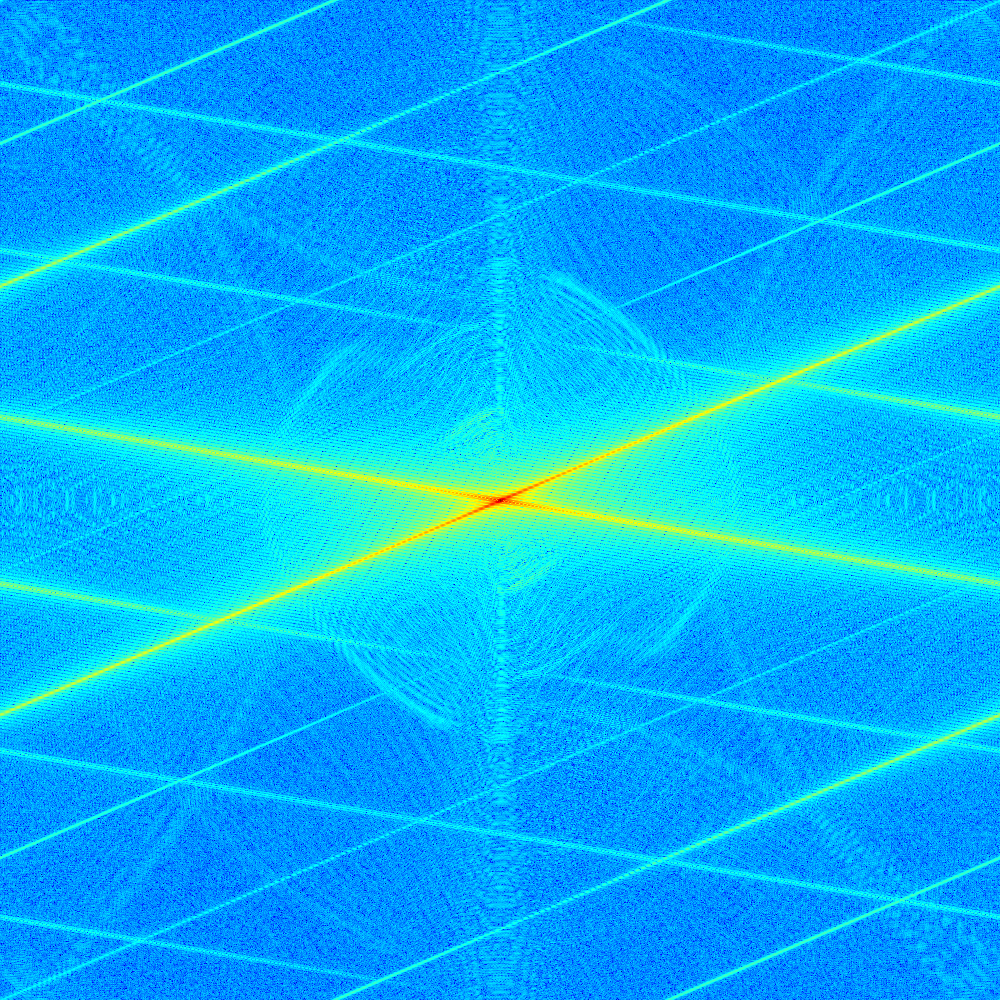
\includegraphics[width = 5cm]{../Figures/spectral_support/fft_red_and_blue.png}};
		\end{scope}
		
		\draw[->] (-5, 0) -- (5, 0) node[right] {$\xi_s$};
		\draw[->] (0, -5) -- (0, 5) node[above] {$\xi_u$};
		
		% Invisible dummy node for symmetric alignment with caption
		\node[left, opacity = 0] at (-5, 0) {$\xi_s$};
		
		\begin{scope}
			\clip (-5, -5) rectangle (5, 5);
			\draw[scale=1, smooth, domain = -10 : 10, variable = \x, blue] plot ({\x},{ -1 / (- 7 / 3) * \x});
			\draw[scale=1, smooth, domain = -10 : 10, variable = \x, red] plot ({\x},{ -1 / (12 / 2) * \x});
		\end{scope}
		
	\end{tikzpicture}
\end{document}